
\documentclass[12pt]{article}
\usepackage{graphicx}
\usepackage{float}

\graphicspath{ {images/}}


\begin{document}

\title{Music App Usability Report}
\author{Jeff Fennell}
\date{September 2014}
\maketitle

\tableofcontents

\section{Intro}

The purpose of this study was to analyze two of the top music 
applications in existence to determine which has been more 
optimized for user interaction. 15 different instances of tests 
were performed on iTunes and Spotify desktop applications.

The first task the test subjects performed was started on the main 
music library of the application. Users were asked to create a new 
playlist with the title "Hello World".  During the second task, 
users again started on the music library of the application. They 
were then asked to make use of the automated radio, a feature that 
is present in both platforms. Users were asked to start the radio 
and create a station adapted to the artist "Tiesto". The final 
task was to navigate to a pre-created playlist on the application, 
and set the playlist to loop indefinitely. For each of the tasks, 
the amount of time it took each user to complete the task was 
noted, as well as the number and nature of errors. Users were also 
asked questions to determine their level of satisfaction with each 
of the systems.

In order to establish a scale for determining which UI was more 
adapted for interaction, we organized our three metrics into a 
hierarchy in order of importance. Efficiency was rated the most 
important metric, followed by errors, and finally, satisfaction. 
We figured that efficiency and errors were more concrete ways of 
assessing usability, while satisfaction is more subjective and 
therefore, should be assessed more-so as a compliment to the other 
two metrics. Through the course of testing, a clear winner 
emerged. All three metrics for the Spotify platform exceeded those 
of iTunes, and it was therefore decided that Spotify is more 
optimized for user interaction.

\section{Metrics}

\subsection{Efficiency}

Spotify users proved to be more efficient in the first task of 
creating a playlist. The average time to create a playlist in 
Spotify was 11.17 seconds, while the average time to perform the 
same task in iTunes took an average of 16.34 seconds. 4 out of 7 
users testing Spotify actually completed the task faster than the 
quickest iTunes time recorded. 3 out of these 4 Spotify testers 
rated their own familiarity of Spotify as being less than 5 out of 
10. Even when removing these users from the efficiency evaluation, 
the averages for Spotify were lower than those of iTunes. Though 
we did not officially evaluate learnability of a metric, this 
speaks to the learnability of Spotify, as users with little domain 
knowledge of Spotify were able to compete the tasks more quickly 
than those with domain knowledge of iTunes. The highest time 
overall was produced by an iTunes user who rated their domain 
knowledge of iTunes as a 9 out of 10. It took this user 26 seconds 
to create a playlist, a full 7 seconds longer than the slowest 
time recorded by a Spotify tester. The slowest iTunes tester noted 
that iTunes frequently updates the user interface, therefore 
making it difficult to stay familiar with how to use certain 
features of the software.

\begin{figure}[H]
	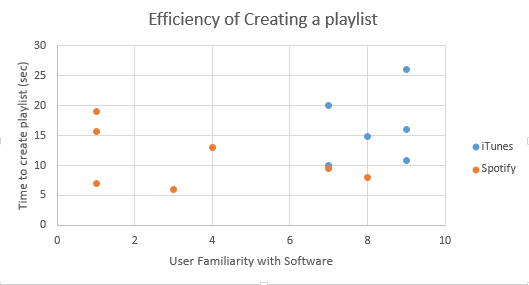
\includegraphics[width=\textwidth]{chart1.png}
	\caption{Average times of completion for each task (lower 
is better)}
\end{figure}

Test subjects again proved to be much more efficient in performing 
the second task in Spotify than in iTunes. The average time to 
complete the task in Spotify was 24.06 seconds. In iTunes, it 
generally took test subjects more than 17 seconds longer to 
complete the task, with the average time being 41.56 seconds. One 
user additionally commented at this stage that starting a radio 
station based on a certain artist in Spotify was "easier than 
iTunes".

The third and final task, starting a playlist and looping it 
indefinitely, designated Spotify as the more efficient platform. 
ITunes testers took an average of 33.52 seconds to navigate to and 
start a playlist looping indefinitely. Spotify users on average 
took a little more than half of the time to perform the same task, 
taking an average of 20.06 seconds.

\subsection{Errors}

In performing the first task, there were relatively few errors. 
Itunes actually did slightly better, with users making only 3 
errors during the first task. Spotify testers collectively made 4 
errors in the course of the first test. In the second test, iTunes 
errors made a total of 6 errors, while Spotify users only made 4. 
On the final task, iTunes testers made 8 errors, while the Spotify 
users only made 2. This puts the total number of errors for the 
iTunes testers at 17 errors, while the number of errors by Spotify 
testers was only 10.

In the second task, one of the errors included attempting to find 
the iTunes radio function through the iTunes store. Another user 
attempted to go through the file menu, and then gave up doing it 
that way, subsequently going through the playlist tab on the 
navigation bar. Another user clicked on the "wishlist" button, 
thinking it would lead them to the radio.

In the third task,  errors generally were related to users not 
being able to determine the functionality of buttons. Users in 
both platforms had a difficult time discerning between the shuffle 
and repeat buttons. Once users figured out which button was the 
repeat button, some of them only clicked it once. This sets not 
the entire playlist to repeat indefinitely, but instead just 
repeats the current song playing indefinitely.

\begin{table}[h]
\centering
\begin{tabular}{lllll}
\hline
            & iTunes & Spotify &  &  \\ \hline
First Task  & 3      & 4       &  &  \\
Second Task & 6      & 4       &  &  \\
Third Task  & 8      & 2       &  &  \\ \hline
Total       & 17     & 10      &  & 
\end{tabular}
\caption{Number of errors made during each task}
\end{table}

\subsection{Satisfaction}

In order to gauge user satisfaction with each of the systems, test 
subjects were asked after each task how satisfied they were with 
the ease of completing the task. Additionally, at the end of all 
three tests, each subject was asked to rate the overall experience 
in using the platform. It is important to notice the difference 
between the user-generated overall, and the average between the 
three tests. The results of the three tests were very close, 
however, the user-reported overall level of satisfaction proved to 
be the tiebreaker, with Spotify again coming out as the winner.


\begin{figure}[H]
	\centering
	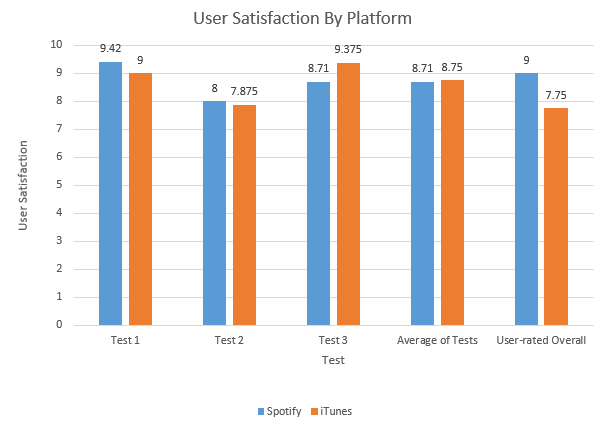
\includegraphics[width=.75\textwidth]{chart2.png}
	\caption{Tester-rated satisfaction with each test, as well 
as an overall level of satisfaction}
\end{figure}

Figure 2 shows the level of satisfaction users experienced for 
each task. Users were only slightly more satisfied with Spotify 
for the first two tests, with an average satisfaction level no 
more than .4 points higher than the iTunes users. In the third 
test, iTunes actually scored significantly higher, with a margin 
of about .6 points separating the two. Regardless of this small 
victory, users still rated the overall experience of Spotify as 
more pleasant than that of iTunes, with a margin of 1.25 points. 
Upon looking at the results, it seems odd that Spotify scored so 
much higher than iTunes overall. Even though the average 
satisfaction for the 3 tests was virtually identical. Possible 
reasons for this difference in rating will be examined in the 
Heuristics section.


\section{Heuristics}

A very strong possible explanation why Spotify testers had higher 
levels of satisfaction with Spotify as a whole lies in the average 
efficiency for each system. As shown in Figure 3, iTunes testers 
took nearly twice as long on average to perform any one task. 
While Spotify users took an average of 18.4 seconds per task, 
iTunes users took a average of 30.47 seconds per task. There is an 
apparent correlation between the amount of time spent performing 
tasks, and the overall satisfaction with the system; the longer a 
user spent performing the same tasks on a system, the lower they 
rated their satisfaction with the system. There are several UI 
style differences that can account for Spotify being a more 
efficient system to use.

\begin{figure}[H]
	\centering
	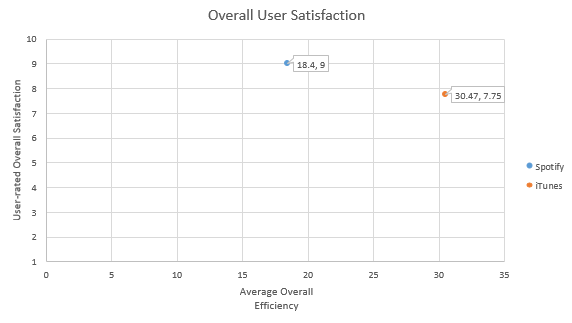
\includegraphics[width=.75\textwidth]{chart3.png}
	\caption{Examining the relationship between average 
efficiency for all 3 tests, and self-rated overall user 
satisfaction with system}
\end{figure}

In examining the style of interaction employed by both Spotify and 
iTunes, some of the reasons that Spotify perform better become 
apparent. One of the more critical components of the Spotify UI to 
note is the use of a vertical, scrollable, navigation column on 
the left-hand side of the screen (shown in figure 4). 

\begin{figure}[H]
	\centering
	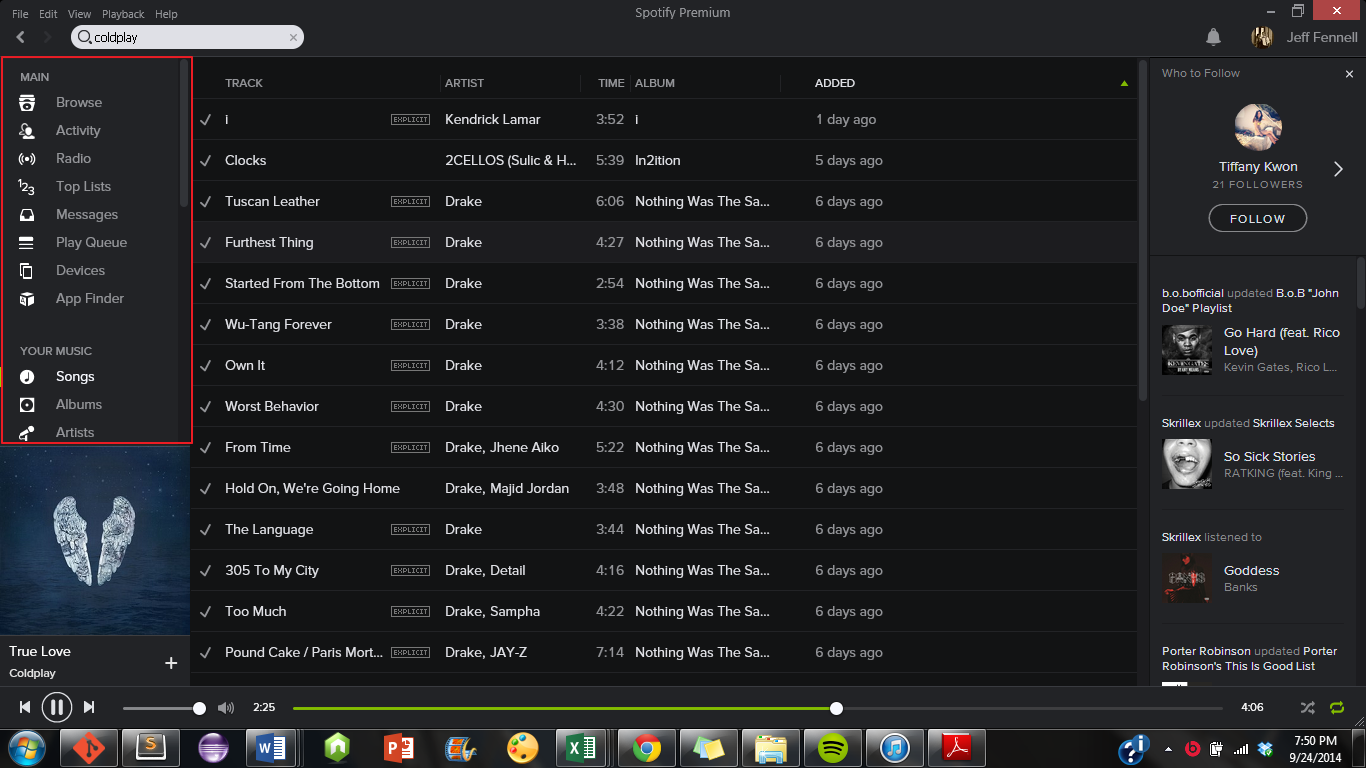
\includegraphics[width=\textwidth]{chart4.png}
	\caption{Spotify employs a navigation column on the left 
hand side of the screen}
\end{figure}

Here, Spotify holds navigation buttons and commonly used function 
buttons all in one column. This navigation bar is a permanent 
fixture in the app, as it remains in place while the user 
navigates through the system. It reduces the number of clicks 
necessary to navigate through the app. Additionally, the fact that 
the left-hand side of the navigation bar touches the corner of the 
window allows the user to navigate to it more quickly. They do not 
have to worry about overshooting the left hand side of the 
navigation bar, as the edge of the screen will stop them. This is 
a direct application of the hotspot concept in Fitts' law.

 All three of the tasks we asked users to carry out actually had 
shortcut buttons in Spotify navigation column. In our first 
test, many of the users utilized the "New Playlist" shortcut in 
the navigation column to create and name a playlist extremely 
quickly. This method creates a playlist in one click, immediately 
allowing the user to type in the name of the new playlist. Even if 
the user uses the file>create playlist> path, it takes only 2 
clicks to create a playlist. Ease of navigation through this menu 
bar was also possible in our second task. There is a link in the 
navigation bar to go straight to the radio function. From there, 
the user must simply type in the name of the artist to start the 
radio station. The first half of the third task was to navigate to 
a playlist, which the user could do from the navigation column.

iTunes, meanwhile, employs a very thin navigation bar that is not 
at the top or the side of the window, but rather, dropped slightly 
towards the center of the screen. This placement and very thin 
size of the navigation bar can allow the user to very easily 
overshoot the navbar when they attempt to click a button. It does 
not have the same hotspot advantage of the navigation column in 
Spotify.

\begin{figure}[H]
	\centering
	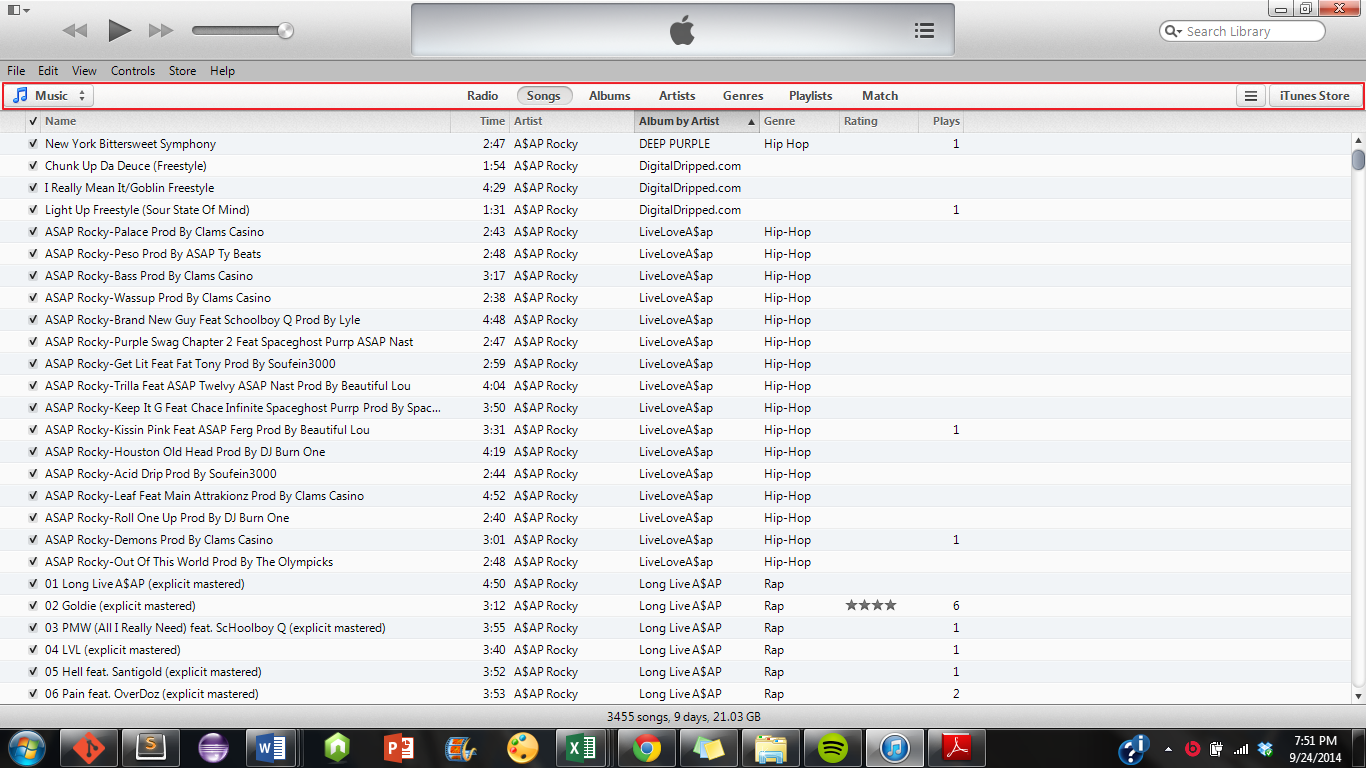
\includegraphics[width=\textwidth]{chart5.png}
	\caption{iTunes employs a horizontal navigation bar with 
two different drop-down menus, as well as navigation tabs}
\end{figure}

While Spotify has navigation shortcuts for common tasks in its 
navigation bar, iTunes does not present the user with as many 
shortcuts. For all three of the tasks, the user in iTunes was 
required to either navigate through the file menu at the top, 
through a series of drop-down menus and button clicks, or navigate 
through separate tabs on the navigation bar, and then click on one 
or more buttons. This inherently is less efficient than the 
Spotify UI, where all of the common shortcuts could be found by 
simply scrolling down the navigation bar. 

By Fitts' law, Spotify is more optimized for user interaction 
because of the way its buttons and navigation items are organized. 
The buttons in Spotify are larger than those of iTunes. Many of 
iTunes' buttons do not have words on them, but rather are glyphs 
representing the tasks, some of which can be confused as one of 
several functions. In addition to just containing symbols, many of 
the Spotify buttons also contain words. This serves two purposes. 
Not only does it give the user a precise description of what 
function the button serves, but also, increases the width of the 
buttons, making them easier to navigate to. Figures 6,7, and 8 
illustrate these points.

\begin{figure}[H]
	\centering
	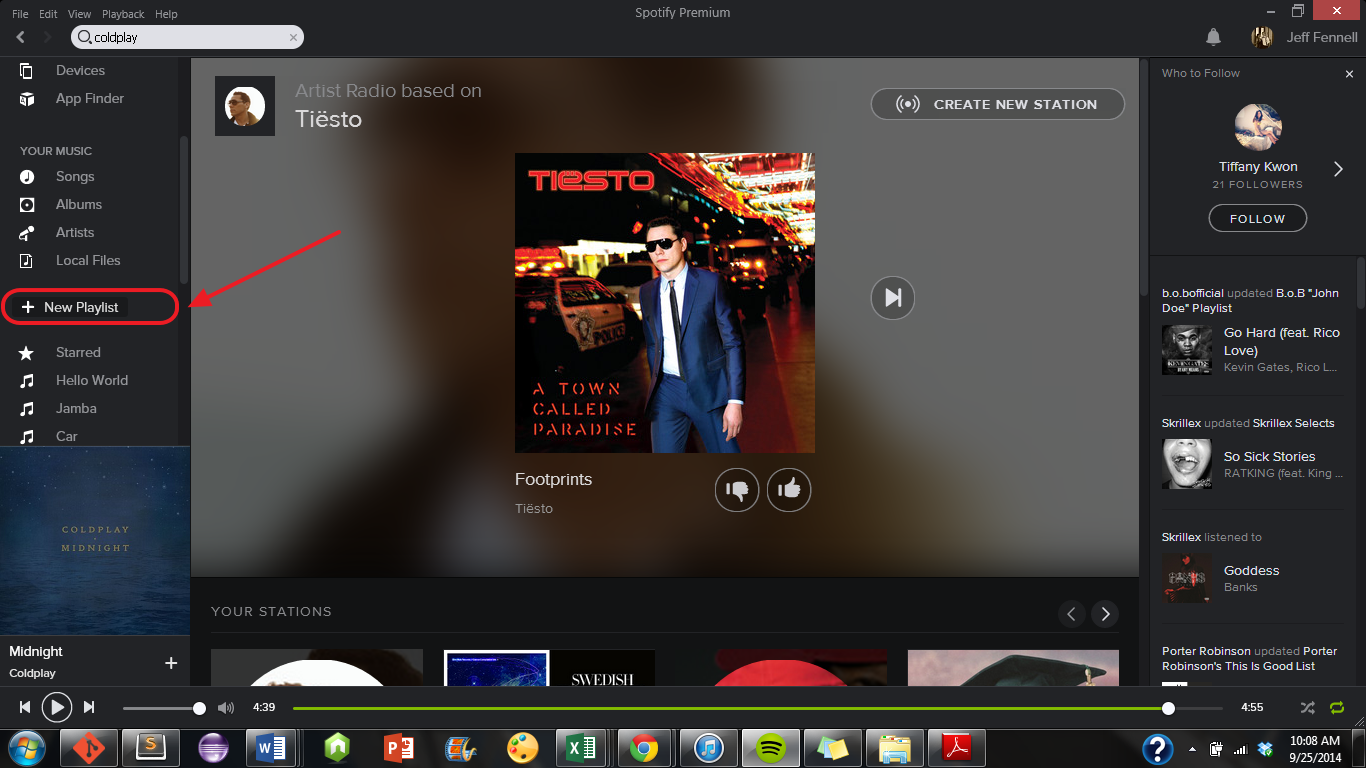
\includegraphics[width=.75\textwidth]{chart8.png}
	\caption{Placement of the "New Playlist" button in the 
navigation column makes it more accessible and easier to click 
than in iTunes (see figure 7) Additionally, it takes only 1 click 
to perform the same task that takes 2 clicks in iTunes (see figure 
8)}
\end{figure}

\begin{figure}[H]
	\centering
	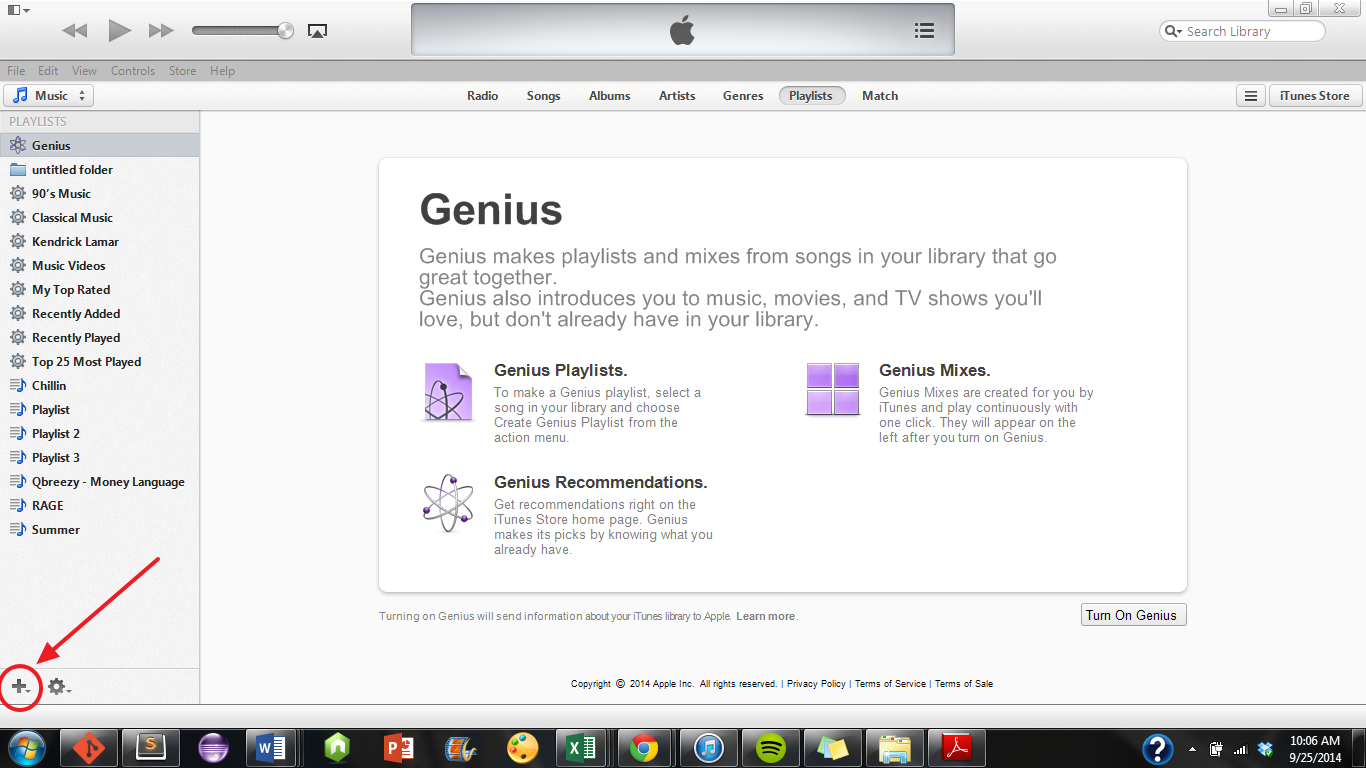
\includegraphics[width=.75\textwidth]{chart7.png}
	\caption{iTunes buttons are generally smaller, contain 
only glyph representations, and as in this instance, are tucked 
into the corner of screen.}
\end{figure}

\begin{figure}[H]
	\centering
	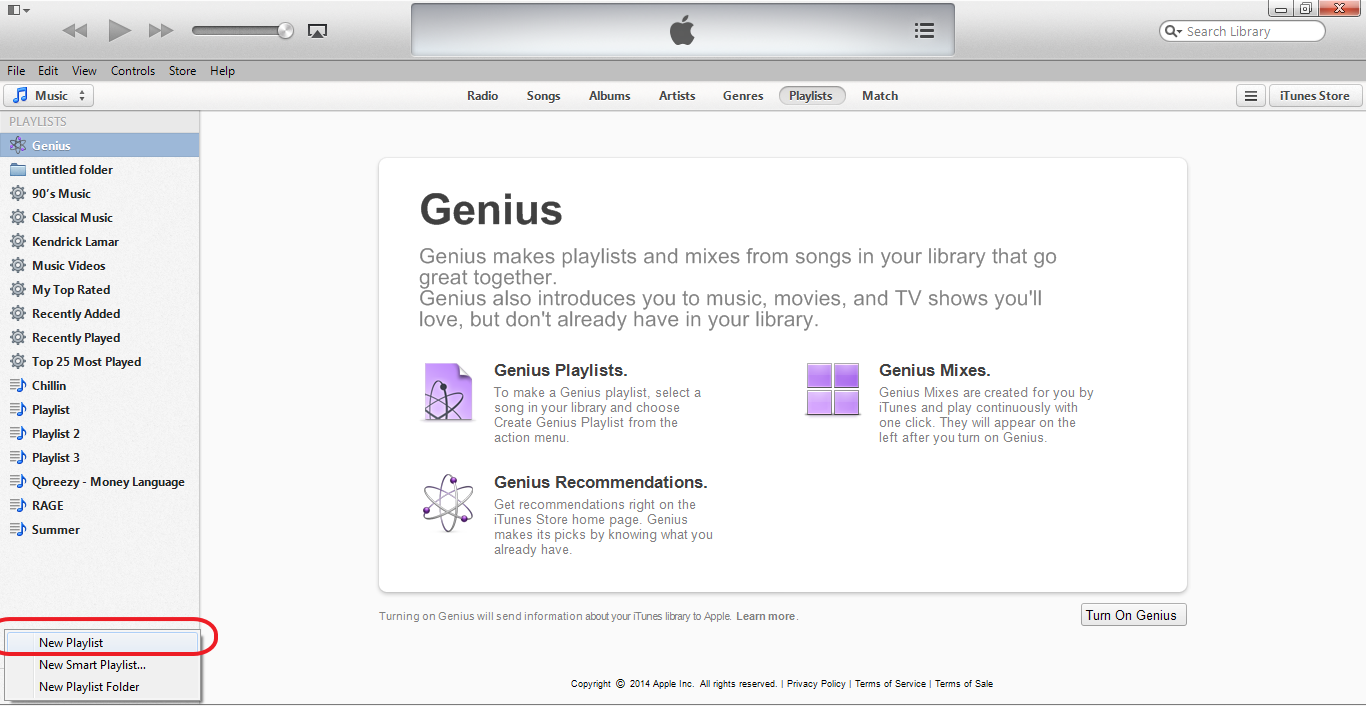
\includegraphics[width=.75\textwidth]{chart9.png}
	\caption{The additional click involved in creating a 
playlist}
\end{figure}


 In essence, the buttons in Spotify are more "in your face". This 
is an explanation for why there were fewer errors overall in 
Spotify than in iTunes. There's another feature of Spotify that 
several testers accidentally exploited to increase efficiency. 
When hovering over the shuffle and repeat buttons, a pop-up 
appears with the description of the button. Several testers 
hovered over the buttons hesitantly, only to find that the 
subsequent pop-up allowed them to discover the purpose of the 
button.

Another subtle component of Spotify that possibly contributes to 
the level of user satisfaction is the presence of spinners. When 
switching between different modules of Spotify, a spinner pops up 
indicating to the user that the module is loading. This does not 
happen in iTunes. When you attempt to navigate from the main music 
library to the radio, for instance, the app appears to be stagnant 
until the radio module has loaded. This is actually in defiance of 
apple's design guidelines  for desktop applications. In the design 
guidelines, apple tells the developer to  "be responsive" to user 
inputs, encouraging the app to give feedback about its state as 
soon as possible. This also defies Tognazzini's first principles 
for interaction design, which is to provide the user feedback with 
some kind of spinner if the wait time is less than or equal to 2 
seconds.

Another explanation of why iTunes is a more usable system involve 
one of Tognazzini's first principles, the concept of Visible 
Navigation. Tognazzini's principle is to create a UI that requires 
as simple of a mental map as possible. The goal is to make the 
user effectively feel that they are staying in one place, with the 
UI doing the work of bringing the content to the user. Spotify 
does a much better job at this than iTunes does. Spotify's UI 
revolves around the navigation bar on the left, the social updates 
column on the right, and a content section in the middle. All 
three of these components are stationary, so the content on them 
does not change upon switching modules. These components of the UI 
leave only a small portion of the screen that changes each time a 
different module is navigated to: the content section. ITunes, 
meanwhile, only has one stagnant component in its UI: the menu and 
navigation bars at the top of the screen, which collectively take 
up much less room on the screen than the stationary Spotify 
components. Upon navigating modules in iTunes, much more of the 
screen changes composition, therefore requiring the user to 
remember much more complex mental maps of the UI layout. All of 
these differences in design approach point out Spotify as the more 
user-friendly system.

\end{document}
